%
% Sección de autenticación de mensajes, capítulo de antecedentes.
% Proyecto Lovelace.
%

\section{Códigos de Autenticación de Mensaje (MAC)}

La información presentada a continuación puede consultarse con más profundidad
en las siguientes referencias
\cite{DBLP:series/isc/DelfsK07, menezes, mac_patel}.

Las funciones \gls{gl:mac} son la técnica simétrica
estándar utilizada tanto para la autenticación como para la protección de la
integridad de los mensajes. Dependen de unas llaves secretas que son
compartidas entre las partes que se van a comunicar; cada una de las
partes puede producir el \gls{gl:mac} correspondiente para un mensaje
dado. Como se explica a continuación, los \gls{gl:mac} pueden ser
obtenidos mediante cifrados de bloque, cifrados de flujo o de funciones
hash criptográficas.

Las funciones hash con llave cuyo propósito específico es la
\gls{gl:autenticacion_origen} y garantizar la \gls{gl:integridad_datos} del
mensaje son llamadas \gls{gl:mac}. Estas funciones tienen como entrada
una llave secreta $k$ y un mensaje de longitud arbitraria y dan como resultado
un mensaje de longitud $n$.

\begin{equation}
  \label{funcion_hash_mac}
  h_k: \{0, 1\}^* \longrightarrow \{0,1\}^n
\end{equation}

El algoritmo \gls{gl:mac} más usado basado en un cifrado de bloque que
utiliza el modo de operación \gls{gl:cbc} (véase sección~\ref{sec:cbc}).
Cuando \gls{gl:des} es utilizado como el cifrado de bloque $E$, el tamaño
de bloque es de 64 bits y la llave \gls{gl:mac} es de 56 bits.

Otra manera de construir \gls{gl:mac} es mediante un algoritmo
de \gls{gl:mdc} que incluya una llave secreta $k$ como parte de la
entrada. Un ejemplo de esto es el algoritmo MD5-MAC; donde la función de
compresión depende de la llave secreta $k$, que interviene en todas las
iteraciones.

El algoritmo \gls{gl:maa} fue diseñado en 1938 específicamente para
obtener \gls{gl:mac} en máquinas de 32 bits. El tiempo de ejecución
es directamente proporcional a la longitud del mensaje y alrededor de cuatro
veces más largo que el \gls{gl:md4}.

\paragraph{\texorpdfstring{\acrlong{gl:prf}}{Función pseudoaleatoria}}
Es posible generar códigos de verificación mediante el uso de funciones
pseudoaleatorias \gls{gl:prf}. Se define en~\ref{mac:1} el algoritmo para
obtener el código de verificación y en~\ref{mac:2} el algoritmo para verificar
si es correcto o no el \gls{gl:mac}.

\begin{pseudocodigo}[caption={\gls{gl:mac} mediante \gls{gl:prf}, obtener código.},
  label={mac:1}]
    entrada:    llave $k$ y mensaje $m$
    salida:     código de autenticación $t$.
    Sea $F$ una función pseudoaleatoria tal que $F:(K \times X) \rightarrow Y$.
    inicio
      $t := F(k,m)$
      regresar $t$
    fin
\end{pseudocodigo}

\begin{pseudocodigo}[caption={\gls{gl:mac} mediante \gls{gl:prf}, verificar código.},
  label={mac:2}]
    entrada:    llave $k$, mensaje $m$, código $t$.
    salida:     resultado de la verificación $r$.
    inicio
      si $t = F(k,m)$ entonces:
        regresar verdadero
      si_no:
        regresar falso
    fin
\end{pseudocodigo}

\paragraph{CBC-MAC}
Este algoritmo está basado en el modo de operación \gls{gl:cbc} y una función
$F$ que puede ser, por ejemplo, un cifrado por bloques. Se encarga de
cifrar con una llave $l_1$ todo el mensaje $m$, pero lo único que se toma en
cuenta es el último bloque, que es tomado como el código de autenticación
(véase figura~\ref{mac:cbc1}). En algunos casos, se cifra de nuevo, con la misma
función $F$, pero utilizando una llave $l_2$ distinta (véase
figura~\ref{mac:cbc2}).

CBC-MAC es considerado seguro cuando el mensaje $m$ tiene una longitud
múltiplo del tamaño de bloque del cifrado por bloques. Como se le han
encontrado varias vulnerabilidades, algoritmos basados en CBC-MAC han sido
propuestos, tales como el \textit{eXtended CBC} o el \gls{gl:omac}.

\begin{figure}
  \begin{center}
    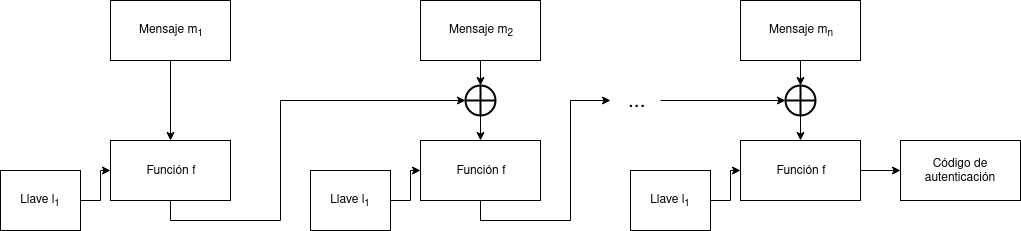
\includegraphics[width=0.9\linewidth]{diagramas/cbcmac.png}
    \caption{Esquema de CBC-MAC simple.}
    \label{mac:cbc1}
  \end{center}
\end{figure}

\begin{figure}
  \begin{center}
    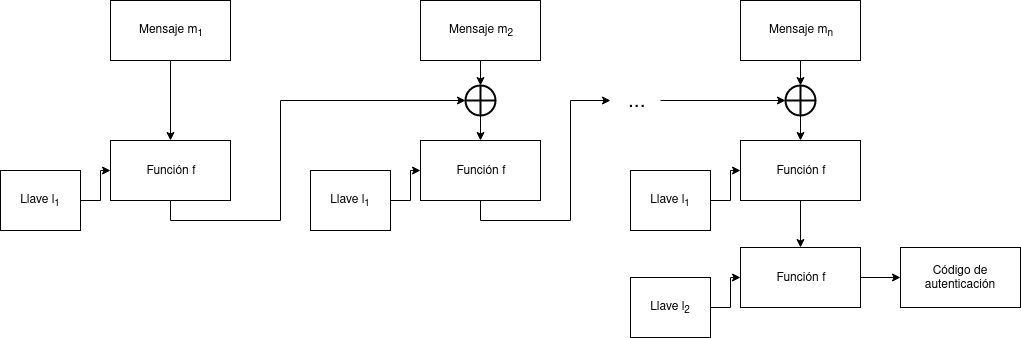
\includegraphics[width=0.9\linewidth]{diagramas/cbcmaclb.png}
    \caption{Esquema de CBC-MAC con el último bloque cifrado.}
    \label{mac:cbc2}
  \end{center}
\end{figure}

% \paragraph{\texorpdfstring{\acrlong{gl:nmac}}{Nested MAC}}
% \gls{gl:nmac} es muy parecido al CBC-MAC, sin embargo, este utiliza una
% función $F$ cuya salida se utiliza como la llave del siguiente bloque. Cuando
% se termina de procesar el mensaje, se le pone un relleno para completar el
% bloque y se cifra una vez más, utilizando una llave $l_2$ (véase
% figura~\ref{mac:nmac}). Es importante cifrar el último bloque usando la
% llave~$l_2$, ya que, de lo contrario, un adversario podría agregar al final
% nuevos bloques a un mensaje interceptado, calculando un nuevo código de
% autenticación, dándole como entrada a la función $F$ el código de autenticación
% original.

% \begin{figure}
%   \begin{center}
%     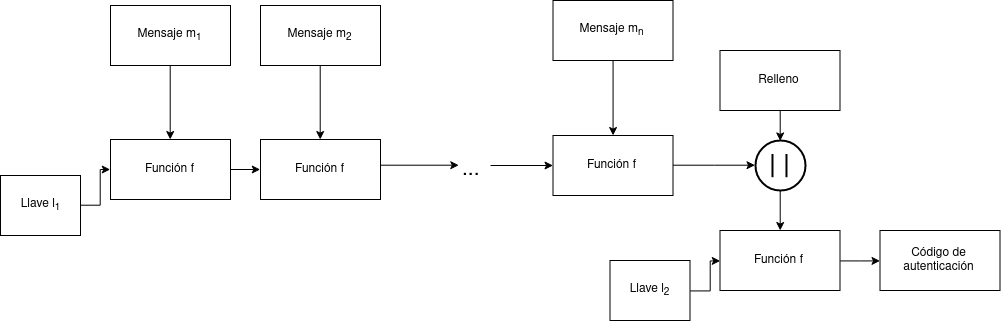
\includegraphics[width=0.9\linewidth]{diagramas/nmac.png}
%     \caption{Esquema de \gls{gl:nmac}.}
%     \label{mac:nmac}
%   \end{center}
% \end{figure}

% \paragraph{\texorpdfstring{\acrlong{gl:cmac}}{Cipher-based MAC}}
% Parecido al algoritmo CBC-MAC, \gls{gl:cmac} utiliza una función $F$ y dos
% llaves ($l_1$ y $l_2$); sin embargo, en vez de utilizar $l_2$ para el segundo
% cifrado, se concatena con el último bloque del mensaje (véase
% figura~\ref{mac:cmac}); entre estos dos elementos ($m_n$ y $l_2$), se agrega una
% secuencia de relleno para poder diferenciarlos. Este paso impide que nuevos
% bloques sean agregados.

% El algoritmo \gls{gl:omac}1 es equivalente al \gls{gl:cmac} y, en 2005, se
% convirtió en una recomendación por el \gls{gl:nist}.

% \begin{figure}
%   \begin{center}
%     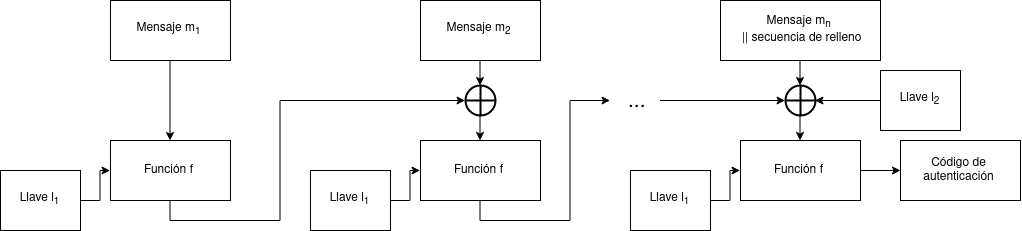
\includegraphics[width=0.9\linewidth]{diagramas/cmac.png}
%     \caption{Esquema de \gls{gl:cmac}.}
%     \label{mac:cmac}
%   \end{center}
% \end{figure}

% \paragraph{\texorpdfstring{\acrlong{gl:pmac}}{Parallel MAC}}
% \Gls{gl:pmac} utiliza dos llaves ($l_1$ y $l_2$) y dos funciones
% ($F_p$ y $F_f$); además, a diferencia de los algoritmos descritos anteriormente,
% \gls{gl:pmac}, tal como lo indica su nombre, puede ser ejecutado paralelamente
% mediante el uso de hilos, pues para procesar un bloque $b_x$ no es necesario
% $b_{x-1}$.

% La llave $l_1$ y un contador $c_i$ se cifran utilizando la función
% $F_p$, la salida es agregada al mensaje $m_i$ con una $XOR$; después, se cifra
% esta salida mediante la función $F_f$ y la llave $l_2$. Cuando se han procesado
% todos los bloques, todas las salidas de $F_f$ se combinan mediante una operación
% $XOR$ y el resultado es cifrado nuevamente mediante $F_f$, que hace uso de
% $l_2$ (véase figura~\ref{mac:pmac})

% Una de las ventajas de \gls{gl:pmac}, es que permite actualizar un bloque $b_x$
% fácilmente, sin tener que recalcular la salida de $F_P$ para todos los demás.
% Es importante que la función $F_p$ sea mucho más rápida que la función $F_f$.

% \begin{figure}
%   \begin{center}
%     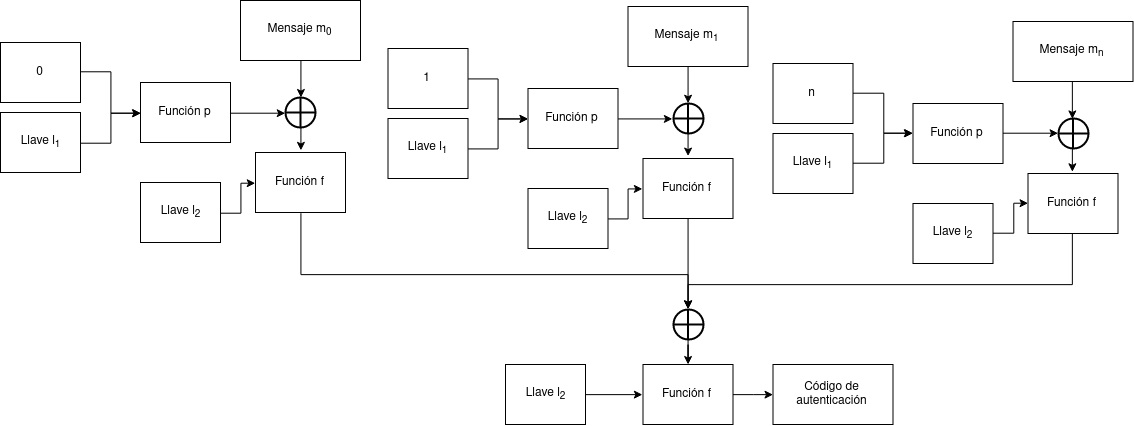
\includegraphics[width=0.9\linewidth]{diagramas/pmac.png}
%     \caption{Esquema de \gls{gl:pmac}.}
%     \label{mac:pmac}
%   \end{center}
% \end{figure}

% \paragraph{\texorpdfstring{\acrlong{gl:omac}}{One-time MAC}}
% Este algoritmo, similar a \gls{gl:libreta_de_un_solo_uso}, es, generalmente,
% más rápido que los algoritmos basados en funciones \gls{gl:prf}. En~\ref{mac:3}
% se define el algoritmo para obtener el código de autenticación. La verificación
% del código se realiza similar a como se mostró en el algoritmo~\ref{mac:2}.

% \begin{pseudocodigo}[caption={MAC mediante \textit{One-time} MAC.},
%   label={mac:3}]
%     entrada:    llaves $l_1$, $l_2$ que se encuentran en el intervalo $[1,q]$
%                 mensaje $M = m_L m_L-1 \dots m_1$
%     salida:     código de autenticación $t$.
%     Sea $P$ una función tal que $P(m, x) = m_Lx^L + \dots + m_1x$.
%     Sea $q$ un primo de aproximadamente $2^{128}$.
%     inicio
%       $t := (P(m, l_1) + l_2) \mod q$
%       regresar $t$
%     fin
% \end{pseudocodigo}

\paragraph{\texorpdfstring{\acrlong{gl:hmac}}{Keyed-Hashed MAC}}
Similar a \gls{gl:nmac}, este algoritmo utiliza una función $h$ \gls{gl:owhf}
para producir códigos de autenticación (véase figura~\ref{mac:hmac}).
Tiene tres parámetros: $relleno_e$, $relleno_s$ y una llave $l$; los primeros
dos se encargan de modificar la llave secreta $l$, por lo que se recomienda que
los valores que asumen cambien lo más posible a $l$ mediante la función $h$.

Este algoritmo es ampliamente utilizado, por ejemplo, se encuentra presente en
los protocolos \gls{gl:ssl} y \gls{gl:ssh}.

\begin{figure}
  \begin{center}
    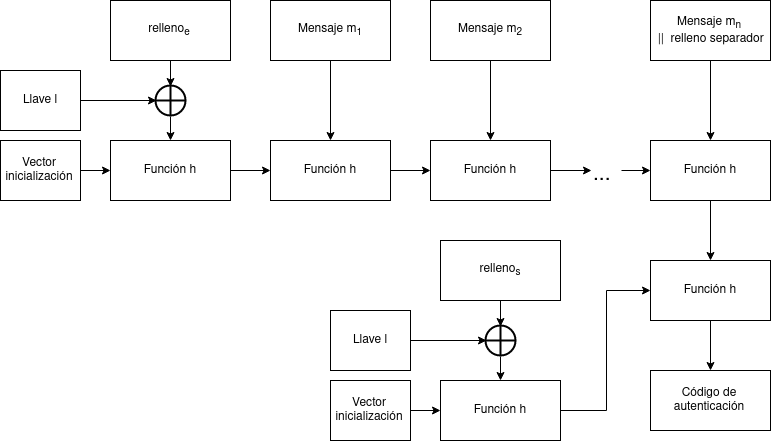
\includegraphics[width=0.9\linewidth]{diagramas/hmac.png}
    \caption{Esquema de \acrshort{gl:hmac}.}
    \label{mac:hmac}
  \end{center}
\end{figure}
